% Fundamentals / environment and related work: 1/3
% comment on employed hardware and software
% describe methods and techniques that build the basis of your work
% review related work(!)

\chapter{Background and Related Work}\label{ch:background}\glsresetall
\section{Cryptocurrency}\label{sec:cryptocurrencies}
% What is cryptocurrency???
Cryptocurrencies are digital or virtual assets, and they use cryptography as a security and consistency mechanism~\cite{investopedia_cryptocurrency, P&D_to_the_moon}. The majority of cryptocurrencies are decentralized systems built on \emph{blockchain} technology, a public tamper proof transaction ledger. With the blockchain, any arbitrary person can verify the consistency of transactions without linking them to real-world identities. Satoshi Nakamoto is the founder of the first and most prevailing cryptocurrency from 2009, namely Bitcoin. In recent years, the number of other cryptocurrencies called \emph{altcoins} have emerged, and at the time writing, there are now over $2000$ different cryptocurrencies~\cite{coinmarketcap}. The altcoins describe themselves as better substitutes as Bitcoin face various complications which \autoref{sec:blockchain} details. Besides Bitcoin, other popular cryptocurrencies are Ripple, Ethereum, XRP, and Litecoin.

% Incentive
Traditional payment systems suffer from the inherent weakness of the trust based model. Completely non-reversible 
transactions are not possible since financial institutions cannot avoid mediating disputes. With the possibility of reversal, the need for trust spreads making merchants prompt customers for their confidential~\cite{bitcoin}. In contrast, cryptocurrency transactions are irreversible, Bitcoin defines an electronic payment as a chain of digital signatures, each transfer are digitally signed with the previous transaction~\cite{bitcoin, ethereum_white}. Cryptocurrency systems are pseudonymous; the public sees all the transactions, but without linking them to real-world identities.

\begin{figure}[ht]
    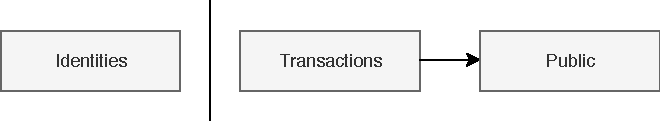
\includegraphics[width=\textwidth]{cryptocurrency_model.pdf}
    \caption{Privacy model for Bitcoin and the majority of altcoins (Source: \cite{bitcoin}).}
    \label{fig:cryptocurrency_model}
\end{figure}

% Issues
Problems originate with the privacy model of Bitcoin and the majority of altcoins, see \autoref{fig:cryptocurrency_model}. According to \cite{bitcoin_regulation}, the emergence of cryptocurrencies has raised significant concerns about potential illegal activities, such as terrorism and money laundering, customer theft and fraud. The expansion of cryptocurrencies may also threaten the traditional money issuance system, question the role of banks and other financial institutions in funds transfers and present a risk for the financial stability in general.

\subsection{Blockchain}\label{sec:blockchain}
% What is a blockchain???
A blockchain~\cite{bitcoin_book} is an ever growing list of blocks, equivalent to a list \ac{adt}~\cite{bitcoin_book}. Blocks in a blockchain consists of data and a \emph{hash pointer}, a reference to and a cryptographic hash of the previous block, see \autoref{fig:blockchain}. Whereas a regular pointer makes it possible to retrieve a blocks location in memory, a hash pointer also makes it possible to verify the integrity of the data. With other words, it is possible to check if the data within a block have changed after the creation of it. In the context of cryptocurrency, blocks contain metadata and a series of transactions.

\begin{figure}[ht]
    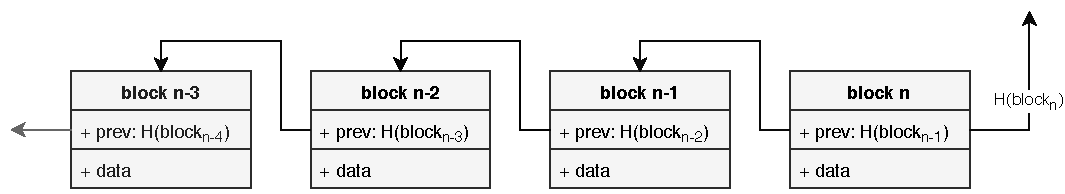
\includegraphics[width=\textwidth]{blockchain.pdf}
    \caption{Abstract view of a blockchain}
    \label{fig:blockchain}
\end{figure}

% Miners and PoW
For nodes (miners) in cryptocurrency systems to solve the double-spending problem and agree on the succeeding block of pending transactions, they all must agree on a single block that comes next in line in the blockchain. The majority of cryptocurrencies use the consensus protocol \ac{pow} to elect the next block, which we define as follows: Miners collect broadcasted pending transactions into a block; they are fussy and exclusively pick the transactions with the highest fees~\cite{trends_fee, trans_fee}. Then, the miners must play a cryptographic puzzle. They start hashing the new block with the hash of the previous block until the digest is below a defined threshold. Each try is pseudo-stochastic, so it requires indefinite attempts, and miners can flip a bit in the block-field \emph{nonce}, so they do not reuse the same digest. The first miner to solve the puzzle gets a minting reward and has to sign the blocks and broadcast it to the other miners which add the new block into the blockchain. Statistically, systems that use \ac{pow} remain their integrity as long as honest nodes possess more than $50\%$ of the total hashing rate in the system.
% Possibly add some inline definitions and functions for properly formalize it.
% NEED TO FIX: 
%   Each try is pseudostochastic so it... 


% Propegation time
The Bitcoin protocol defines the issuing rate of new blocks to be approximately ten minutes. After the immense interest in cryptocurrency, the amount of miner has skyrocket which results in high electricity expenditure and longer verification time of transactions due to the slower propagation time of blocks. Bitcoin miners electrical consumption alone can power five million U.S households and the emission of CO$_2$ for producing the required electricity is $275$ kilogram per transaction~\cite{bitcoin_power}. As the number of miners escalates, the longer propagation time of blocks, thus, the time-gap of where two or more block being proposed and integrated by miners at the same time expand~\cite{trans_fee}. When the miners have a different vision of the blockchain, they have created a \emph{branch}. Any branch is fixable though producing the longest branch as the \ac{pow} protocol looks at the longest branch as the true main branch. The blocks that are mined but was cut off from the main branch are invalid and called \emph{orphaned block}. And because of the possibility of orphaning, a rule of thumb in verification of Bitcoin transactions is to wait until a block with your payment is confirmed (buried under other blocks) six times~\cite{bitcoin_verification_1, bitcoin_verification_2} which is around one hour.

\subsection{Exchanges}\label{sec:exchanges}
% what are exchanges?
Cryptocurrency exchanges are centralized online platforms where traders can exchange cryptocurrency for another cryptocurrency or fiat\footnote{Money made by the government\cite{fiat}}. They are typically market makers that take \emph{bid-ask} spreads as transaction commissions for their services or charge fees as a matching platform~\cite{norton_rose}. Currently, they lack regulation\footnote{Application of law by the government} which makes them not trustworthy and susceptible to price manipulation schemes and con artists~\cite{exchange_scammers, exchange_scammers_2}. There are over $200$ different cryptocurrency exchanges where some of the most appealing are Coinbase, Binance, Bittrex, and Poloniex~\cite{exchange_best_1, exchange_best_2}, where Binance has a monthly trading volume of more than \$$20$ billion~\cite{coinmarketcap_exchange}.

% trading pairs
Cryptocurrency exchanges list various symbol pairs denoting a \emph{base} and \emph{quote}. The currency pairs compare the value of one currency to another - the base currency versus the quote. It indicates how much of the quote currency is needed to purchase one unit of the base currency~\cite{investopedia_cryptocurrency}. Furthermore, exchanges categorize symbol pairs in markets, where the quote are typically the name of the market. For example, to trade Ethereum (ETH) for Bitcoin (BTC), the symbol pair "ETH/BTC" is in the Bitcoin market along with countless other symbol pairs.

% tokens
Trades on cryptocurrency exchanges are with \emph{tokens} which makes them off-blockchain~\cite{exchange_off_chain}, but in return, there is no need for verification as trades happening instantly. However, traders seemingly prefer to use multiple exchanges simultaneously, and transaction between exchanges are registered on the cryptocurrency's blockchain, see \autoref{fig:exchanges}. Exchanges are contradictory to the incentive of cryptocurrencies as they are decentralized systems while exchanges are centralized, but still, $99\%$ of cryptocurrency trades happen on exchanges~\cite{coinsutra}.
%% NEED TO REWRITE

\begin{figure}[ht]
    \centering
    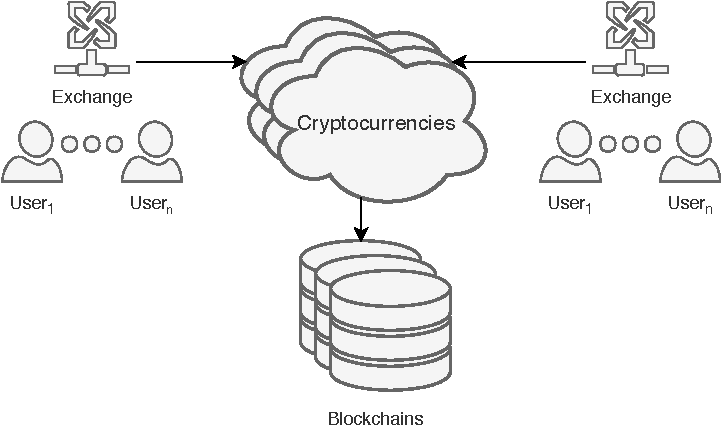
\includegraphics[width=\textwidth]{exchanges.pdf}
    \caption{Cryptocurrency exchanges ecosystem}
\label{fig:exchanges}
\end{figure}

\subsubsection{Market data}
% rest api
Before the internet, trading, in general, took place over the phone, in the post-internet age, trading takes effect over an exchange's \ac{api}~\cite{exchange_api} allowing software to pull data and interact with the exchange. \acp{api} are useful analytics and for traders who have algorithmic models that are fueled by live data and need to issue orders within milliseconds.

\subsubsection{OHLCV}
Graphical illustrations of price movements for specific time intervals goes by the name \emph{kline} or \emph{candlestick} chart. Such graphs utilize a set of \acp{ohlcv} points, describing the trading trends in a time window. \autoref{tab:ohlcv} illustrates a candle in its crude form, and \autoref{fig:pd-gxsbtc} shows processed \acp{ohlcv} values making a candlestick chart. The top and bottom wicks represent the highest and lowest trade price respectively in the time interval, while the color portrays whether the closing price was higher or lower than the opening price~\cite{P&D_to_the_moon}. Candles can define trading trends in any time interval, but exchange’s \ac{api} mostly allows a discrete selection of timeframes that commonly range from one minute to several days.
\begin{table}[ht]
    \centering
    \begin{tabular}{ c c c c c c }
        \hline
        \textbf{Timestamp} & \textbf{Price} & & & & \textbf{Trading volume} \\
        \cline{2-5}\\
                  & \textbf{Open}  & \textbf{High} & \textbf{Low} & \textbf{Close} & \\
        \hline
        2019-06-01 23:59:59 & $2006.2$ &  $2061.3$ & $1926.2$ & $1984.1$ & $216304.7$\\
        \hline
    \end{tabular}
    \caption[Structure - \Acf{ohlcv}]{shows the structure of an \acp{ohlcv} value. The volume presents the number of assets that were traded over a period. The price field denotes the highest and lowest price that was recorded, as well as the price from where the period started (open) to where it ended (close).}
    \label{tab:ohlcv}
\end{table}



\subsubsection{Order Book}
% Order book
% Level 1 & Level 2
An order book also aliased market depth is an electronic list of buying and sell orders on an exchange for a specific symbol pair, see \autoref{tab:order_book}~\cite{investopedia_depth}. Sell orders are in an \emph{asks} list in a descending order while buy orders are arranged descendingly in a \emph{bids} list~\cite{invest_order_book, coincodex_order_book}. The order book is dynamic and constantly change throughout the day as traders are issuing new orders. There are many ways to interpret an order book; for instance, a massive imbalance of buy orders versus sell orders may indicate a price increase due to buying pressure~\cite{invest_order_book}.
\begin{table}[ht]
    \centering
    \begin{tabular}{c c| c c}
        \hline
         \textbf{Asks} & & \textbf{Bids} & \\
         \textbf{Price} & \textbf{Volume} & \textbf{Price} & \textbf{Volume}\\
         \hline
         [$0.028$ ... $0.14$] & [$12.4$ ... $3.1$] & [$0.027$ ... $0.018$] & [$56.4$ ... $1.45$]\\
         \hline
    \end{tabular}
    \caption[Structure - Order book]{shows the structure of an order book. The left side (askers) includes the quantity of coins that are buyable, while the right side (bidders) are bids that are waiting to be matched against buyable coins. }
    \label{tab:order_book}
\end{table}

\subsection{Pump-and-Dump}\label{sec:pd}
A \ac{pd} scheme is a type of fraud in which the offenders accumulate a commodity over a period, then artificially inflate the price through means of spreading misinformation (pumping), before selling off what they bought to unsuspecting buyers at the higher price (dumping)\cite{P&D_to_the_moon}. After the emergence of cryptocurrency trading, \ac{pd} has become a popular legitimate price manipulation scheme among scammers, who leach assets from the misinformed. Two researchers at the Imperial College London revealed that on average, at least two \ac{pd} schemes are carried out daily, producing \$$7$ million in daily trading volume~\cite{P&D_MIT_crypto}. Price increases of up to 950\% have been witnessed, demonstrating the amount of potential profit~\cite{P&D_cointelegraph}.

\begin{figure}[ht]
    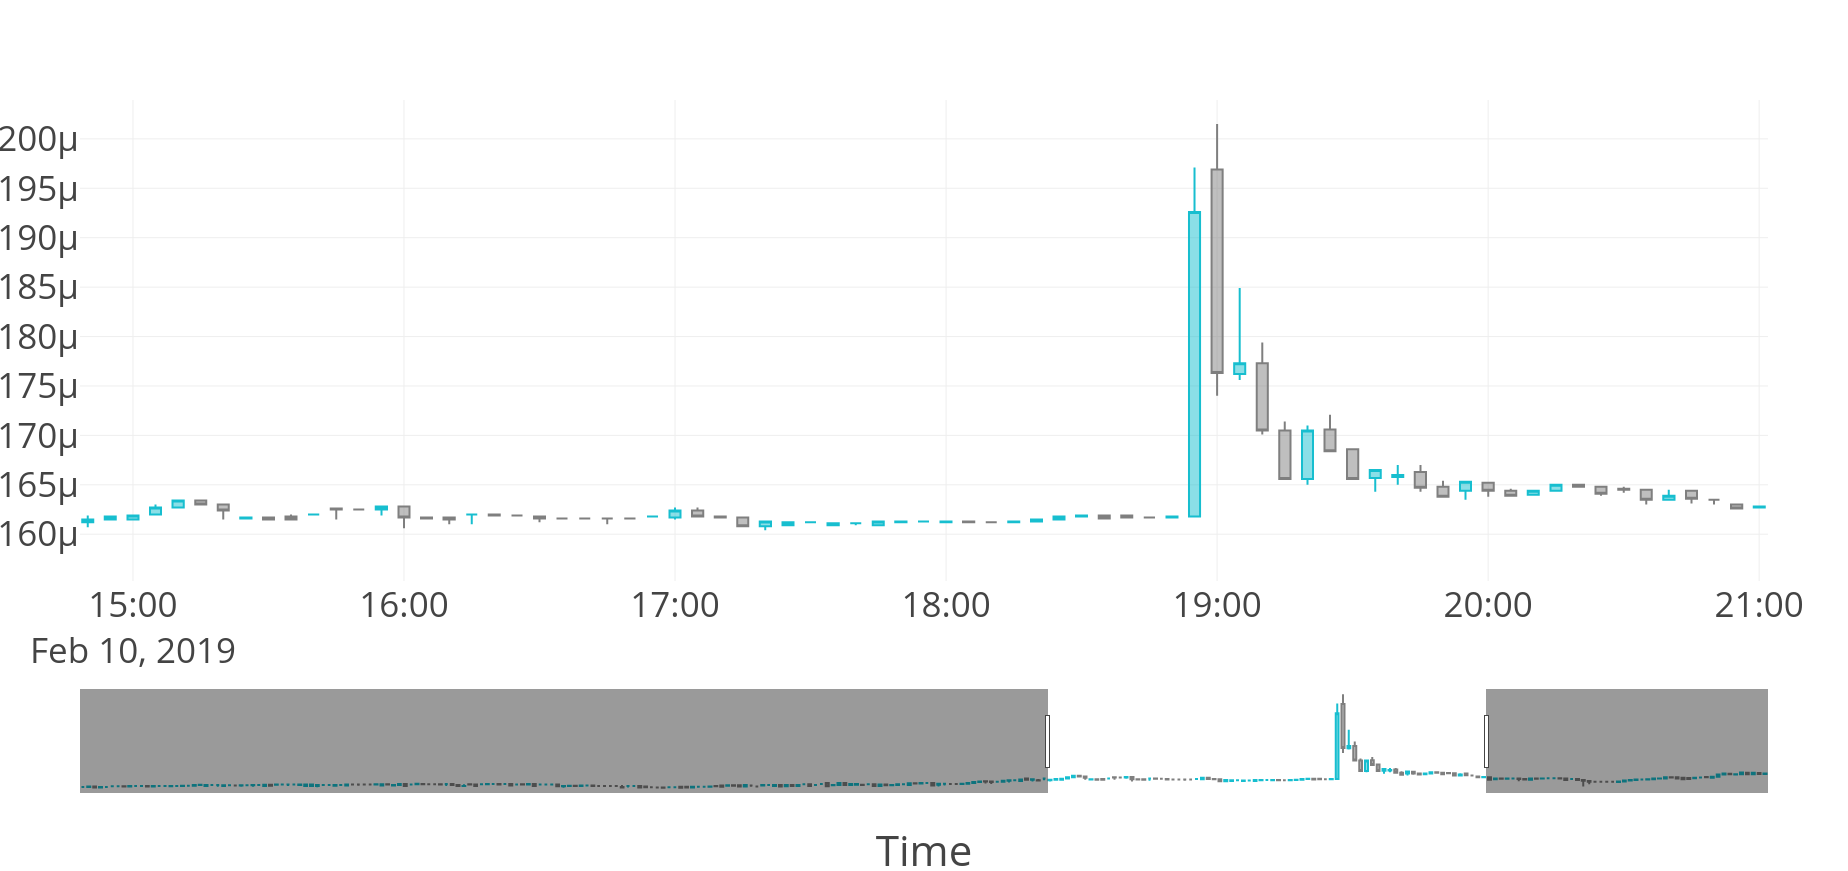
\includegraphics[width=\textwidth]{GXS-BTC.png}
    \centering
    \caption{\ac{pd} organized by the group Crypto Pump Island on 2019-02-10 19:00. The target symbol was GXS/BTC on the exchange Binance.}
    \label{fig:pd-gxsbtc}
\end{figure}

% stock market
On the modern stock market, \ac{pd} schemes are internet-based focusing on \emph{penny} or \emph{microcap} stocks, which are smaller companies that do not comply with the standards to being listed on the larger exchanges~\cite{stock_bouraoui, stock_temple, P&D_anatomy}. Microcap stock exchanges are not held to the same standard of regulation, which implies that there are usually not as much information about the companies that are listed making them easier to manipulate~\cite{P&D_to_the_moon}. Misinformation about the stocks are usually spread through email spam which have a net positive effect on the stock price~\cite{stock_bouraoui}. It is illegal to run price manipulation schemes on regulated markets, and there are multiple cases where participants in a \ac{pd} are prosecuted~\cite{P&D_to_the_moon}.

% cryptocurrency market
There is a slightly different approach of \acp{pd} on the cryptocurrency market. The pump is a coordinated, intentional, short-term increase in the demand of a symbol pair~\cite{P&D_anatomy} organized by dedicated groups. These groups are often public channels in chat applications like Discord or Telegram and are joined by naive traders, who believe they will become wealthy in a short amount of time. The number of members in some of the prominent groups have peaked at circa $200,000$~\cite{P&D_the_outline}.

\subsubsection{Pump Groups}\label{sec:pump_groups}
% Group setup
In the cryptocurrency market, \ac{pd} organizers (admins) create groups in encrypted chatting application such as Telegram and Discord. They advertise themselves through social media platforms and forums~\cite{P&D_anatomy, P&D_scheme} as exciting groups that ensures profit with little or no risk of losing assets. The group admins start to organize \ac{pd} when the group typically consists of over $\numprint{1000}$ optimistic traders~\cite{P&D_anatomy}. Only the admins are allowed to post messages in the group restricting regular members to just see the messages posted by the admins; this functionality is enabled by the admins to avoid member interference~\cite{P&D_anatomy}.

% Accumulate
Before a \ac{pd}, the group admins announce details regarding it a few days ahead. The information they provide is the exact time and date, the quote which is more or less always Bitcoin, and the exchange. With the information, the member can buy sufficient funds on the targeted exchange in advance~\cite{P&D_anatomy}. The same day the \ac{pd} is scheduled, the admins purchase a commodity in the base coin over a period without raising the price. And they send out countdowns and reminds the members of previous successfully \acp{pd} to motivate them to participate, and the "rules" during the upcoming \ac{pd}. According to \cite{P&D_anatomy}, the typical rules are.

\begin{enumerate}
    \item Make sure to buy fast.
    \item \emph{Shill}\footnote{Cryptocurrency jargon for "promote" or "advertise" coin.} the announced coin on social media to attract outsiders.
    \item \emph{HODL}\footnote{Cryptocurrency jargon for Hold.} the coin for several minutes to give outsiders the possibility of joining.
    \item Sell in pieces at profit, not in chunks.
\end{enumerate}

% pump-and-dump
When the admins announce the coin, each member tries to be the first to buy the published coin to ensure profit before the inevitable inflation. If they are to slow, they might buy at the peak and are unable to make a profit. The pressure of being the first is high because the coin peak within seconds to max ten minutes~\cite{P&D_the_outline, P&D_anatomy}. After they have bought a significant amount of the coin, they shill, in an attempt to trick outsiders into buying it, allowing them to sell easier~\cite{P&D_anatomy}. The misinformation varies, but some common tactics include false news stories, non-existent projects, fake partnerships, or fake celebrity endorsements~\cite{P&D_the_outline}. Simultaneously, the admins encourage the members to hold while they sell off what they bought earlier on that day making them maximize their profit before the inevitable price dump. As soon as the first fall in price appears, the members start to panic-sell. If the price dips below the start price, the second wave of traders buys to bounce the price up to where it began allowing them to gain a small profit~\cite{P&D_anatomy}.

% post pump
Minutes to hours later, when the coin recover to its initial state. The admins publish results that showcases the members impact and the potential profit. \autoref{fig:chat_pump} shows real messages from \ac{pd} organized by the pump group Crypto Pump Island, and the \autoref{fig:pd-gxsbtc} shows the impact.

Nevertheless, in the end, only the admins and a few members are profiting from a \ac{pd} while the majority are loosing. So why are there still people enthusiastic about partaking a \ac{pd}, given the risk of being ripped off by the admins? Because people believe that there are greater fools out there, who would buy the coins at an even higher price than their original purchase price~\cite{P&D_anatomy}. The greater fools theory is also what thrives many other price manipulation schemes~\cite{dissecting}.
\begin{figure}[ht]
    \begin{leftbubbles}
    30 minutes left to pump on Binance. $\color{gray}_{\text{18:30}}$
    
    15 minutes left to pump on Binance. $\color{gray}_{\text{18:45}}$
    
    5 minutes left to pump on Binance. $\color{gray}_{\text{18:55}}$
    
    Next post will be the coin name. $\color{gray}_{\text{18:55}}$
    
    Coin name: gxs $\color{gray}_{\text{19:00}}$
    
    Go go go.. $\color{gray}_{\text{19:00}}$

    Buy and Hold. And sell in parts $\color{gray}_{\text{19:01}}$
    
    Amazing... $\color{gray}_{\text{19:02}}$
    
    Hope everyone gets profit.
    Good holding $\color{gray}_{\text{19:05}}$
    \end{leftbubbles}
    \caption{Messages from the telegram group Crypto Pump Island on 10 February 2019.}
    \label{fig:chat_pump}
\end{figure}

\subsubsection{Characteristics}
Detection of \ac{pd} schemes requires insights in their operations to have the ability to identify patterns that occur during a \ac{pd}. \autoref{tab:pd_characteristics} which is defined by two researchers at the University College London \cite{P&D_anatomy} summarizes some of the fundamental similarities and differences with respect to the target, tactic and timescale of traditional penny stock and cryptocurrency \ac{pd} schemes. It clearly shows that traditional and cryptocurrency \ac{pd} schemes target the same type of markets, but the tactic and timescale differ. The lack of trust among members in the pump groups can explain the short timescale of cryptocurrency \acp{pd}, as they all want their piece of the cake and sell as soon as they profit instead of holding. Spreading of misinformation must happen in real-time because of the short time pressure.

\begin{table}[ht]
    \centering
    \begin{tabular}{l c c}
    \hline
     &\textbf{Traditional} & \textbf{Cryptocurrency}\\
    \hline
     Target   & Low market cap & Low market cap \\
              & Low volume     & Low volume \\
              & Low price      & Low price \\
              & Lack of reliable information & Lack of reliable information\\
              \\
    Tactic    & Misinformation & Real-time\\
              & Privately organized & Public or private group scams\\
              \\
    Timescale & Medium (days to weeks) & Short (Seconds to minutes)\\
    \hline
    \end{tabular}
    \caption[\acf{pd} characteristics]{Characteristics of traditional and cryptocurrency \ac{pd} schemes. (Source: \cite{P&D_to_the_moon}). }
    \label{tab:pd_characteristics}
\end{table}

Using the characteristics, the same two researchers \cite{P&D_anatomy} formulated criterion's that can be helpful when detecting \ac{pd} patterns in exchange data (\autoref{tab:pd_indicators}). The indicators are split into \emph{breakout} and \emph{reinforcers}. The breakout indicators point out patterns that are present during the beginning of a \ac{pd}. And the reinforcers are external aspects to strengthening our confidence in an alleged \ac{pd}. The signs $(+)$ and $(-)$ are a confidential boost; the former denotes an increase while the latter denotes a decrease. The volume and price factors in the breakout indicators are discussed with an estimation window, referring to a collection of previous data points, of some user-specified length~\cite{P&D_anatomy}.

\begin{table}
    \centering
    \begin{tabular}{p{0.33\textwidth} p{0.33\textwidth} p{0.33\textwidth}}
    \hline
    \textbf{Breakout indicators} &\textbf{Real-time indicators} & \textbf{Post-pump indicators}\\
    \hline
    Volume & Has the volume at the current data point been significantly higher than in the estimation window? & Was there a decline in volume after the event window where a pump was detected?\\\\
    Price & Has the price at the current data point been significantly higher than in the estimation window? & Was there a decline in price after the event window where a pump was detected?\\\\
    \end{tabular}
    
    \begin{tabular}{p{0.33\textwidth} p{0.66\textwidth}}
    \hline
    \textbf{Reinforcers} &\textbf{Temporal dimension}\\
    \hline
    Market cap & Is the market cap of the coin relatively low? $(+)$\\\\
    Number of exchanges & Whether the coin is listed on multiple exchanges and the indicators only spike on one $(+)$\\
                        & Whether the coin is listed on multiple and the indicators spike on multiple exchanges (neutral)\\
                        & Whether the coin is not listed on multiple exchanges $(+)$\\\\
    Symbol pair         & Whether the coin is trading for BTC or some other cryptocurrency $(+)$\\
                        & Whether the coin is trading for USD or some other fiat currency $(-)$\\
    Time                & Whether the coin is start on the hour or half hour and last a few minutes$(+)$\\
    \hline
    \end{tabular}
    \caption{Indicators of \ac{pd} per temporal dimension and indicator type. (Source: \cite{P&D_to_the_moon, P&D_anatomy})}
    \label{tab:pd_indicators}
\end{table}
 
\newpage
\section{Deep Learning}
\Acf{ml} is a fast-growing field in computer science, and it refers to the ability to make a computer recognize specific patterns in data using various complex algorithmic models. In the broader field of \ac{ml}, recent years have witnessed a proliferation of deep neural networks, with fantastic results across various application domains. Deep learning is a subset of machine learning that achieves excellent performance and flexibility that surpasses conventional \ac{ml} algorithms~\cite{mike_voets, dl_anomaly}.

\begin{quote}
    \emph{A breakthrough in machine learning would be worth ten Microsoft.} - Bill Gates
\end{quote}

As \Ac{ml} has become a buzzword and categorized as state of the art and "the solution" for every kind of problem, it is important to remember that \ac{ml} is not always the optimal solution for every type of problem. There are certain cases where rule-based solutions perform better than \ac{ml}, cases, where we can directly predict values by using simple rules, computations, or predetermined steps that are easily programmable~\cite{aws}. So when should we use \ac{ml}? According to \cite{aws}, we should use \ac{ml} in following situations:

\begin{itemize}
    \item When tasks cannot be adequately solved using deterministic rule-based solutions. A considerable number of factors like features, patterns, correlated features, etc., can influence the answer. When rules depend on too many factors, and many of these rules overlap or need to be tuned very finely, it quickly becomes complicated to define these rules accurately.
    \item When tasks do not scale, e.g., manual detection of spam mail which will be a tedious process if there are millions of emails. \ac{ml} solutions are effective at handling large-scale problems.
\end{itemize}

Algorithms in \Ac{ml} are commonly subdivided into two major paradigms, \emph{unsupervised} and \emph{supervised} learning. In supervised learning, the algorithms require data and prior knowledge of each sample, called \emph{labels} or \emph{ground truth}, and the algorithms in unsupervised learning need only data. There are two terms that circumstance under supervised learning, regression, and classification. Both share the same concept of using data to make a prediction. Classification problems refer to the ability to recognize a discrete set of classes, while a regression problem, estimates a value from input data.

Deep learning allows computational models that are composed of multiple processing layers to learn representations of data with various levels of abstraction~\cite{lecun2015deep}. Each layer's output is the connected layer's input~\cite{mike_voets}. These deep learning models learn like many other \ac{ml} models, by iteratively minimizing a cost function to adjust its internal parameters (weights) using a training data set. When the weights are appropriately adjusted, it evaluates its performance by making classifications on a test data set. \ac{ml} model facilitates the automatic classification of data, which, when deployed, removes the need for a person to classify the data manually~\cite{mike_voets}.

Considering the amount of \ac{pd} events in trading data, a \ac{pd} can be categorized as an anomaly as it exists significant more regular trading activity than \acp{pd}. The choice of a deep neural network architecture in anomaly detection methods primarily depends on the nature of input data. One distinguishes Input data into sequential (e.g., voice, text, music, time series, protein sequences) and non-sequential data (e.g., images)~\cite{dl_anomaly}. Cryptocurrency sources produce sequential data, more specifically \emph{time series} data. Time series data are linearly ordered sequence of values of a variable at equally spaced time intervals~\cite{stat_handbook}. Anomaly detection in multivariate time series data is a challenging task, but \ac{rnn} and \ac{lstm} networks are shown to perform well in detecting anomalies within time series~\cite{dl_anomaly}.

\subsection{Neural Networks}
A traditional \ac{ml} model do not have any perception of its previous predictions, and when working with non-sequential data, it is not needed. However, when having sequential data, a point only yields information within a specific context. For example us humans do not start our thinking from scratch every second. When we read an essay, we understand each word based on our understanding of previous words. We do not throw everything away and start thinking from scratch again. Our thoughts have persistence~\cite{colah}. The same concept can we apply to the cryptocurrency market, we do not know if the price of a coin has increased unless we know the previous values, and the purpose with a \ac{pd} is to raise the price. Hence, if we were to detect \ac{pd} without having any perception of change in price, both humans and \ac{ml} algorithms would have a hard time detecting them.

\begin{figure}
    \centering
    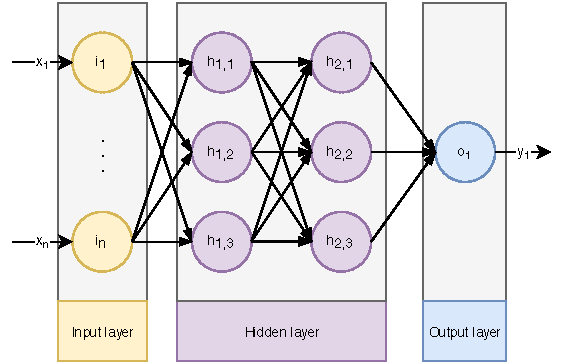
\includegraphics[width=\textwidth]{nn.pdf}
    \caption{Structure of an artificial neural network}
    \label{fig:nn}
\end{figure}

An \ac{ann} (\autoref{fig:nn}) is a powerful learning model, and it is one of the most frequently used model~\cite{hunt1992neural} that achieve state-of-the-art results in a wide range of supervised learning tasks~\cite{lipton2015critical}. A vanilla \ac{ann} does not have a perception of previous samples. Thus, it can not catch the trend in data. \ac{rnn} is a type of network that has an internal state (memory) allowing it to set samples in a specific context. Yet, a standard \ac{rnn} suffers from the \emph{vanishing} and the \emph{exploding} gradient problems~\cite{bengio1994learning}. \ac{lstm} is a type of \ac{rnn} that solves said problems by using standard cells in addition to memory cells. The structure of \ac{lstm} networks is similar to \autoref{fig:nn}, and compose of three different layers, called \emph{input layer}, \emph{hidden layer}, and \emph{output layer}.

The cells in the input layer are mostly passive, meaning they do not make any calculations nor modifying the data somehow, and the number of cells is equal to the number of features in the data. Their task is to duplicate their received data and propagate it every cell in the first column in the hidden layer.

The hidden layer has no interaction with the outside of the network. Hence, the name hidden~\cite{data_science, stanford}. This layer can comprise multiple layers with an arbitrary number of cells but with more cells the complexity of the network increase. Each cell algorithmic structure depends on the type of network we want to build(\ac{ann}, \ac{rnn}), \emph{perceptron} and \emph{lstm} are two cells that are used, where \ac{lstm} is good at detecting pattern in sequential data, while a perceptron are good at detecting pattern in non-sequential. However, all cells have at least two things in common; they all have an input and an output, and the output from one cell is the succeeding cells in the input of the next layer. 

The cells in the output layer take input from the last set of cells in the hidden layer. Their algorithmic structure is similar to the cells in the hidden layer, but their output is also the final prediction from the network.

\newpage
\section{Related Work}\label{sec:related_work}
% Stock Price Manipulation Detection Based on Mathematical Models
An article from ICACI\footnote{International Conference on Advanced Computational Intelligence} 2016, \cite{P&D_stock_price_manipulation} presented a model that detects \ac{pd} schemes on the stock market and did so with $88\%$ accuracy. The article describes how badly \ac{pd} schemes are executed and organized. And from the patterns a \ac{pd} scheme leaves behind, the article proposed mathematical definitions based on level $2$ order book data with a depth of $10$ to generate a training set consisting of buying and sell orders. The researchers implemented a feedforward neural network and trained it with the generated dataset, and achieved an accuracy of precisely $88.28\%$.

% Cryptocurrency Pump Predictions: A novel approach to identifying Pump-and-Dump Scheme
Two students from Standford Unversity recreated the stock market model~\cite{P&D_stock_price_manipulation} and made it compatible with cryptocurrency exchanges in 2017. In their work, they used level $1$ order book data to generate a training set to train a neural network and a Support Vector Machine. They labeled the dataset by identifying \acp{pd} by comparing a market's price movement to BTC. The final test results of their models was $78.13\%$ with Support Vector Machine and $82.5$\% with the neural network. 

The following articles two were recently published, both in late November 2018.

% To the moon: defining and detecting cryptocurrency pump-and-dumps
Kleinberg and Kamps from the University College London\cite{P&D_to_the_moon} defined specific patterns in \acp{pd} and how they differ from the stock market. Also, they proposed a novel anomaly detection approach based on a set of criteria for locating suspicious transactions patterns on cryptocurrency exchanges. The most balanced parameters for their algorithm resulted in about $1.6$ \acp{pd} per market for a total of $2150$ over $20$ days of data. Moreover, $75\%$ of the alleged pump were to found to have corresponding price dumps. They state in their conclusion; Ultimately, it is the hope that the information presented in this paper is useful for further research into the detection of this fraudulent scheme~\cite{P&D_to_the_moon}. For us, this article proved to be indeed helpful.

% The Anatomy of a Cryptocurrency Pump-and-Dump Scheme
Another two researchers in London, but from the Imperial College London, wrote an article~\cite{P&D_anatomy} that analyzes features of pumped markets and market movement of coins before, and after \acp{pd}. They implemented a predictive Random Forest model that gives the likelihood of each possible coin being pumped prior to the actual pump event. With an AUC of the ROC curve of over 0.9, the model exhibits high accuracy and is indicative of the “pumpability” of coins~\cite{P&D_anatomy}. This article has actually received a lot of recognition and attention~\cite{P&D_MIT_crypto, P&D_cointelegraph, P&D_UTB} on media platforms that covers cryptocurrencies.
